\documentclass{beamer}
\usepackage[utf8]{inputenc}
\usepackage{graphicx, epsfig}
\usepackage{amsmath,mathrsfs,amsfonts,amssymb}
\usepackage{floatflt}
\usepackage{epic,ecltree}
\usepackage{mathtext}
\usepackage{fancybox}
\usepackage{fancyhdr}
\usepackage{multirow}
\usepackage{enumerate}
\usepackage{epstopdf}
\usepackage{multicol}
\usepackage{algorithm}
\usepackage[noend]{algorithmic}
\usepackage{tikz}
\usepackage{blindtext}
\usetheme{default}%{Singapore}%{Warsaw}%{Warsaw}%{Darmstadt}
\usecolortheme{default}

\setbeamerfont{title}{size=\Huge}
\setbeamertemplate{footline}[page number]{}

\setbeamertemplate{section in toc}[sections numbered]


\makeatletter
\newcommand\HUGE{\@setfontsize\Huge{35}{40}}
\makeatother    

\setbeamerfont{title}{size=\HUGE}
\beamertemplatenavigationsymbolsempty

% latin bold lower
\newcommand{\ba}{\mathbf{a}} 
\newcommand{\bc}{\mathbf{c}} 
\newcommand{\be}{\mathbf{e}} 
\newcommand{\bh}{\mathbf{h}} 
\newcommand{\bp}{\mathbf{p}} 
\newcommand{\bt}{\mathbf{t}} 
\newcommand{\bs}{\mathbf{s}} 
\newcommand{\bu}{\mathbf{u}} 
\newcommand{\bv}{\mathbf{v}} 
\newcommand{\bw}{\mathbf{w}} 
\newcommand{\bx}{\mathbf{x}} 
\newcommand{\by}{\mathbf{y}} 
\newcommand{\bz}{\mathbf{z}} 

% latin bold upper
\newcommand{\bA}{\mathbf{A}} 
\newcommand{\bB}{\mathbf{B}} 
\newcommand{\bC}{\mathbf{C}} 
\newcommand{\bI}{\mathbf{I}} 
\newcommand{\bJ}{\mathbf{J}} 
\newcommand{\bL}{\mathbf{L}} 
\newcommand{\bM}{\mathbf{M}} 
\newcommand{\bP}{\mathbf{P}}
\newcommand{\bQ}{\mathbf{Q}} 
\newcommand{\bR}{\mathbf{R}} 
\newcommand{\bT}{\mathbf{T}} 
\newcommand{\bU}{\mathbf{U}} 
\newcommand{\bV}{\mathbf{V}} 
\newcommand{\bW}{\mathbf{W}} 
\newcommand{\bX}{\mathbf{X}} 
\newcommand{\bY}{\mathbf{Y}} 
\newcommand{\bZ}{\mathbf{Z}} 

% latin cal upper
\newcommand{\cF}{\mathcal{F}} 
\newcommand{\cG}{\mathcal{G}} 
\newcommand{\cI}{\mathcal{I}} 
\newcommand{\cL}{\mathcal{L}} 
\newcommand{\cM}{\mathcal{M}} 
\newcommand{\cN}{\mathcal{N}} 
\newcommand{\cS}{\mathcal{S}} 
\newcommand{\cT}{\mathcal{T}} 
\newcommand{\cW}{\mathcal{W}} 
\newcommand{\cX}{\mathcal{X}} 
\newcommand{\cZ}{\mathcal{Z}} 

% latin bb upper
\newcommand{\bbE}{\mathbb{E}} 
\newcommand{\bbI}{\mathbb{I}} 
\newcommand{\bbP}{\mathbb{P}} 
\newcommand{\bbR}{\mathbb{R}} 

% greek bold lower
\newcommand{\bepsilon}{\boldsymbol{\epsilon}} 
\newcommand{\btheta}{\boldsymbol{\theta}} 
\newcommand{\blambda}{\boldsymbol{\lambda}} 
\newcommand{\bpi}{\boldsymbol{\pi}} 
\newcommand{\bmu}{\boldsymbol{\mu}} 
\newcommand{\bsigma}{\boldsymbol{\sigma}} 
\newcommand{\bphi}{\boldsymbol{\phi}} 

% greek bold upper
\newcommand{\bSigma}{\boldsymbol{\Sigma}} 

\DeclareMathOperator*{\argmin}{arg\,min}
\DeclareMathOperator*{\argmax}{arg\,max}

\newcommand{\createdgmtitle}[1]{\title[\hbox to 56mm{Deep Generative Models  \hfill\insertframenumber\,/\,\inserttotalframenumber}]
	{Deep Generative Models \\ {\Huge Lecture #1}}
	\author{Roman Isachenko}
	\institute{
\includegraphics[width=0.5cm]{../utils/ozonmasterslogo} \large{Ozon Masters}}
	\date{Spring, 2022}
}

\usepackage{tikz}
\usetikzlibrary{arrows,shapes,positioning,shadows,trees}

\newcommand\myfootnote[1]{%
  \tikz[remember picture,overlay]
  \draw (current page.south west) +(1in + \oddsidemargin,0.5em)
  node[anchor=south west,inner sep=0pt]{\parbox{\textwidth}{%
      \rlap{\rule{10em}{0.4pt}}\raggedright\scriptsize \textit{#1}}};}

\newcommand\myfootnotewithlink[2]{%
  \tikz[remember picture,overlay]
  \draw (current page.south west) +(1in + \oddsidemargin,0.5em)
  node[anchor=south west,inner sep=0pt]{\parbox{\textwidth}{%
      \rlap{\rule{10em}{0.4pt}}\raggedright\scriptsize\href{#1}{\textit{#2}}}};}
      
\AtBeginSection[]
{
	\begin{frame}{Outline}
		\tableofcontents[currentsection,subsectionstyle=hide]
	\end{frame}
}
\AtBeginSubsection[]{
	\begin{frame}{Outline}
		\tableofcontents[currentsection,currentsubsection]
	\end{frame}
}
\createdgmtitle{14}

\usepackage{tikz}

\usetikzlibrary{arrows,shapes,positioning,shadows,trees}
%--------------------------------------------------------------------------------
\begin{document}
%--------------------------------------------------------------------------------
\begin{frame}[noframenumbering,plain]
%\thispagestyle{empty}
\titlepage
\end{frame}
%=======
\begin{frame}{Recap of previous lecture}
	\begin{block}{Continuous-in-time normalizing flows}
		\vspace{-0.5cm}
		\[
			\frac{d\bz(t)}{dt} = f(\bz(t), t, \btheta); \quad \frac{d \log p(\bz(t), t)}{d t} = - \text{tr} \left( \frac{\partial f (\bz(t), t, \btheta)}{\partial \bz(t)} \right).
		\]
		\vspace{-0.7cm}
	\end{block}
	\begin{block}{Theorem (Picard)}
		If $f$ is uniformly Lipschitz continuous in $\bz$ and continuous in $t$, then the ODE has a \textbf{unique} solution.
	\end{block}
	\begin{block}{Forward transform + log-density}
		\vspace{-0.4cm}
		\[
			\begin{bmatrix}
				\bx \\
				\log p(\bx | \btheta)
			\end{bmatrix}
			= 
			\begin{bmatrix}
				\bz \\
				\log p(\bz)
			\end{bmatrix} + 
			\int_{t_0}^{t_1} 
			\begin{bmatrix}
				f(\bz(t), t, \btheta) \\
				- \text{tr} \left( \frac{\partial f(\bz(t), t, \btheta)}{\partial \bz(t)} \right) 
			\end{bmatrix} dt.
		\]
		\vspace{-0.4cm}
	\end{block}	
	\begin{block}{Hutchinson's trace estimator}
		\vspace{-0.3cm}
		\[
		   \log p(\bz(t_1)) = \log p(\bz(t_0)) - \mathbb{E}_{p(\bepsilon)} \int_{t_0}^{t_1} \left[ {\color{violet}\bepsilon^T \frac{\partial f}{\partial \bz}} \bepsilon \right] dt.
		\]
	\end{block}
	\myfootnotewithlink{https://arxiv.org/abs/1810.01367}{Grathwohl W. et al. FFJORD: Free-form Continuous Dynamics for Scalable Reversible Generative Models, 2018} 
\end{frame}
%=======
\begin{frame}{Recap of previous lecture}
	\vspace{-0.2cm}
	\begin{block}{SDE basics}
		Let define stochastic process $\bx(t)$ with initial condition $\bx(0) \sim p_0(\bx)$:
		\[
			d\bx = \mathbf{f}(\bx, t) dt + g(t) d \bw, 
		\]
		where $\bw(t)$ is the standard Wiener process (Brownian motion)
		\vspace{-0.2cm}
		\[		
			\bw(t) - \bw(s) \sim \cN(0, (t - s) \bI), \quad d \bw = \bepsilon \cdot \sqrt{dt}, \, \text{where } \bepsilon \sim \cN(0, \bI).
		\]
	\end{block}
	\vspace{-0.5cm}
	\begin{block}{Langevin dynamics}
		Let $\bx_0$ be a random vector. Then under mild regularity conditions for small enough $\eta$ samples from the following dynamics
		\vspace{-0.2cm}
		\[
			\bx_{t + 1} = \bx_t + \eta \frac{1}{2} \nabla_{\bx_t} \log p(\bx_t | \btheta) + \sqrt{\eta} \cdot \bepsilon, \quad \bepsilon \sim \cN(0, \bI).
		\]
		will comes from $p(\bx | \btheta)$.
	\end{block}
	The density $p(\bx | \btheta)$ is a \textbf{stationary} distribution for the Langevin SDE.
	\myfootnotewithlink{https://www.stats.ox.ac.uk/~teh/research/compstats/WelTeh2011a.pdf}{Welling M. Bayesian Learning via Stochastic Gradient Langevin Dynamics, 2011}
\end{frame}
%=======
\begin{frame}{Recap of previous lecture}
	\begin{figure}
		\centering
		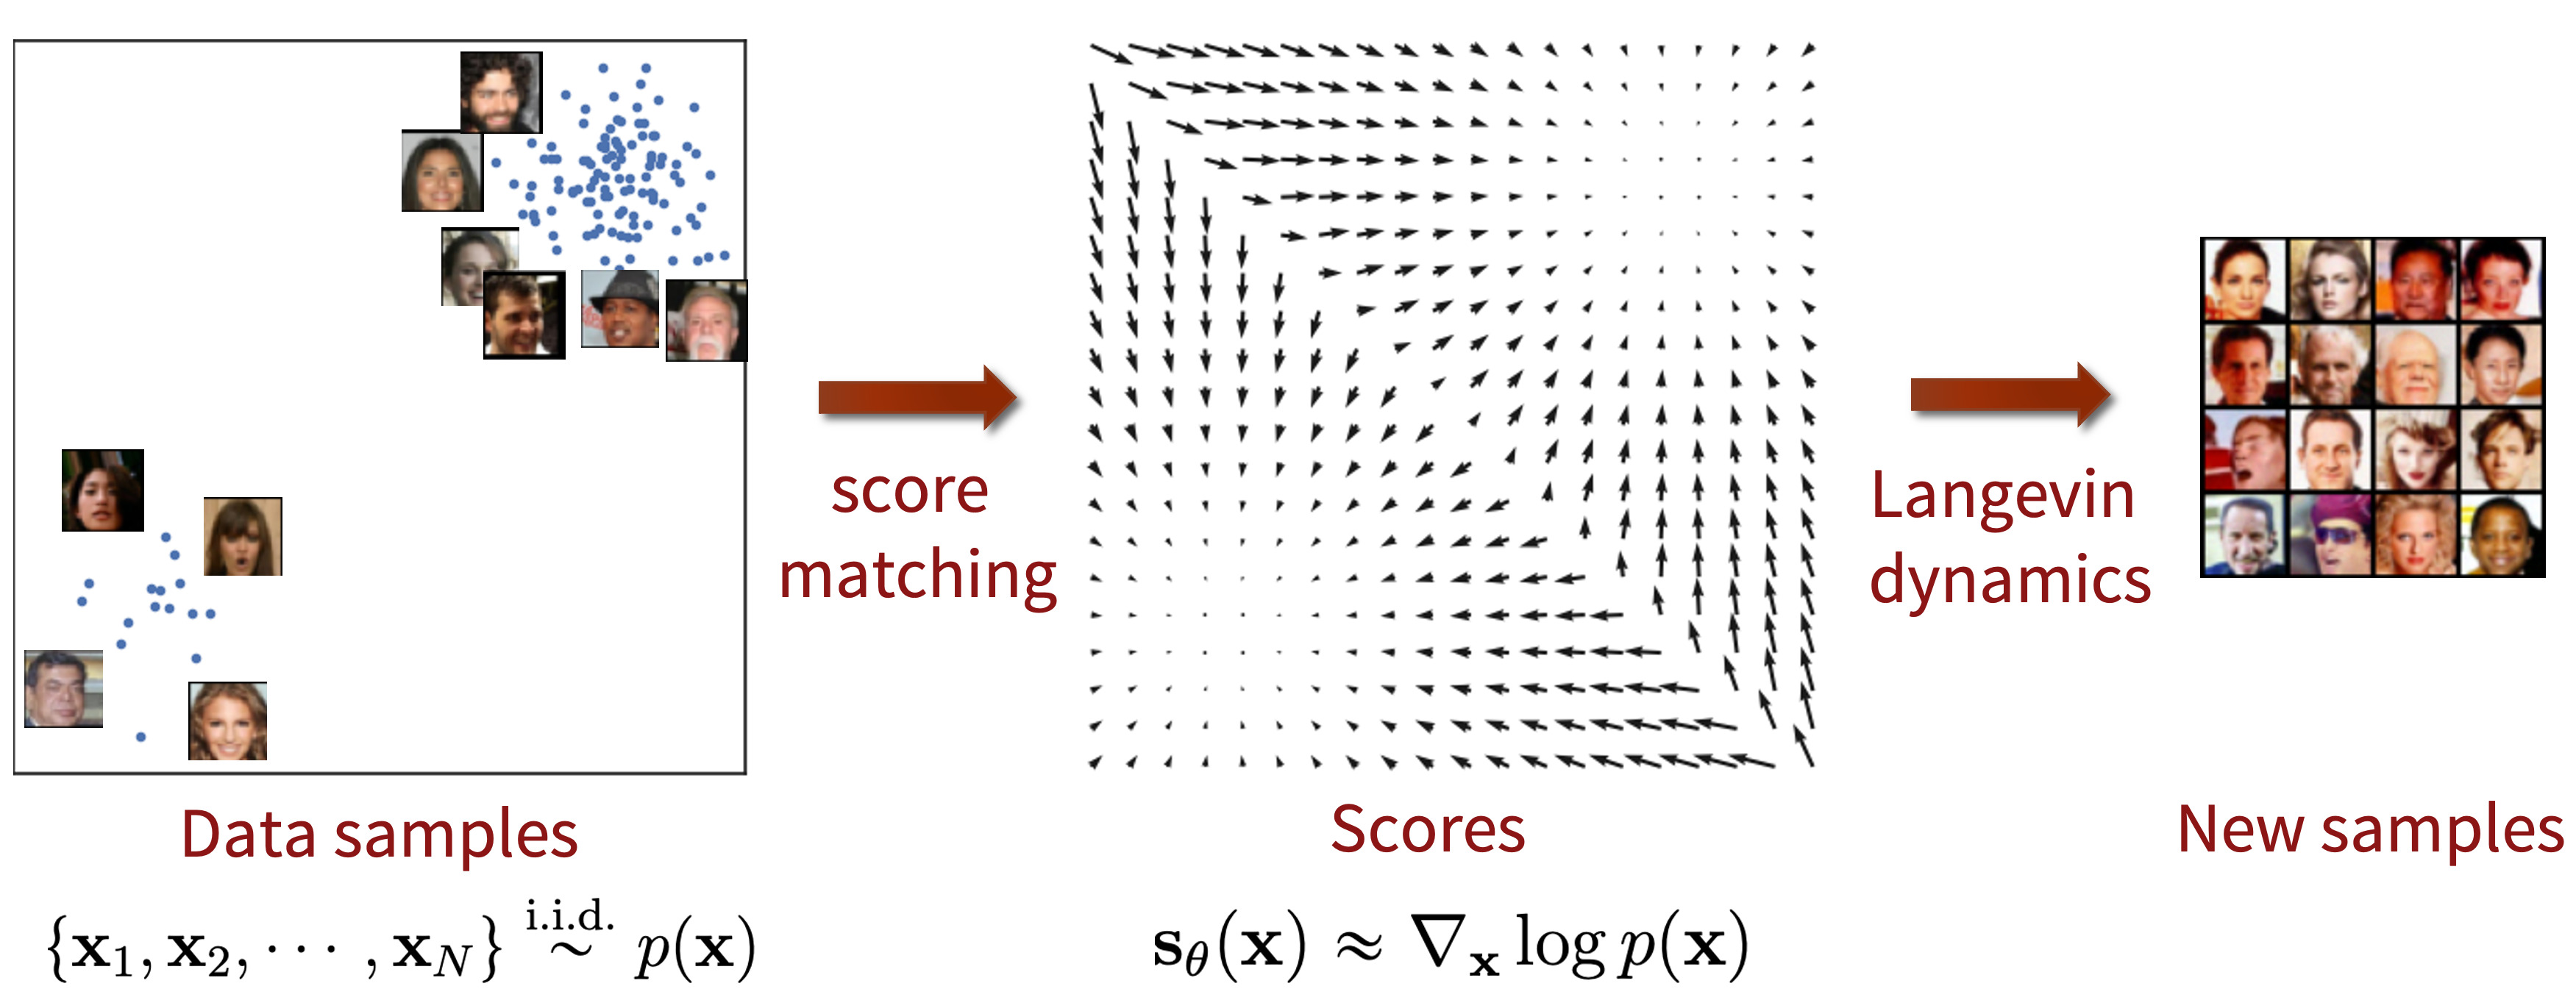
\includegraphics[width=0.75\linewidth]{figs/smld}
	\end{figure}
	\vspace{-0.3cm} 
	\begin{block}{Theorem (implicit score matching)}
		\vspace{-0.6cm}
		\[
		{\color{violet}\frac{1}{2} \bbE_{\pi}\bigl\| \bs(\bx, \btheta) - \nabla_\bx \log \pi(\bx) \bigr\|^2_2} = {\color{teal}\bbE_{\pi}\Bigr[ \frac{1}{2}\| \bs(\bx, \btheta) \|_2^2 + \text{tr}\bigl(\nabla_{\bx} \bs(\bx, \btheta)\bigr) \Bigr]} + \text{const}
		\]
	\end{block}
	\vspace{-0.5cm}
	\begin{enumerate}
		\item {\color{violet}The left hand side} is intractable due to unknown $\pi(\bx)$ -- \textbf{denoising score matching}. 
		\item {\color{teal}The right hand side} is complex due to Hessian matrix -- \textbf{sliced score matching (Hutchinson's trace estimation)}.
	\end{enumerate}
	\myfootnotewithlink{https://yang-song.github.io/blog/2019/ssm/}{Song Y. Generative Modeling by Estimating Gradients of the Data Distribution, blog post, 2021}
\end{frame}
%=======
\begin{frame}{Recap of previous lecture}
	Let perturb original data by normal noise $p(\bx | \bx', \sigma) = \cN(\bx | \bx', \sigma^2 \bI)$
	\vspace{-0.3cm}
	\[
	\pi(\bx | \sigma) = \int \pi(\bx') p(\bx | \bx', \sigma) d\bx'.
	\]
	\vspace{-0.6cm} \\
	Then the solution of 
	\vspace{-0.2cm}
	\[
	\frac{1}{2} \bbE_{\pi(\bx | \sigma)}\bigl\| \bs(\bx, \btheta, \sigma) - \nabla_\bx \log \pi(\bx | \sigma) \bigr\|^2_2 \rightarrow \min_{\btheta}
	\]
	\vspace{-0.5cm} \\
	satisfies $\bs(\bx, \btheta, \sigma) \approx \bs(\bx, \btheta, 0) = \bs(\bx, \btheta)$ if $\sigma$ is small enough.
	\begin{block}{Theorem (denoising score matching)}
		\vspace{-0.8cm}
		\begin{multline*}
			\bbE_{\pi(\bx | \sigma)}\bigl\| \bs(\bx, \btheta, \sigma) - \nabla_\bx \log \pi(\bx | \sigma) \bigr\|^2_2 = \\ = \bbE_{\pi(\bx')} \bbE_{p(\bx | \bx', \sigma)}\bigl\| \bs(\bx, \btheta, \sigma) - \nabla_\bx \log p(\bx | \bx', \sigma) \bigr\|^2_2	
		\end{multline*}
		\vspace{-0.8cm}
	\end{block}
	Here $\nabla_{\bx} \log p(\bx | \bx', \sigma) = - \frac{\bx - \bx'}{\sigma^2}$.
	\begin{itemize}
		\item The RHS does not need to compute $\nabla_{\bx} \log \pi(\bx | \sigma)$ and even more $\nabla_{\bx} \log \pi(\bx)$.
		\item $\bs(\bx, \btheta, \sigma)$ tries to \textbf{denoise} a corrupted sample.
		\item Score function $\bs(\bx, \btheta, \sigma)$ parametrized by $\sigma$. How to make it?
	\end{itemize}
	\myfootnotewithlink{http://www.iro.umontreal.ca/~vincentp/Publications/smdae_techreport.pdf}{Vincent P. A Connection Between Score Matching and Denoising Autoencoders, 2010}
\end{frame}
%=======
\begin{frame}{Outline}
	\tableofcontents
\end{frame}
%=======
\section{Noise conditioned score network}
%=======
\begin{frame}{Denoising score matching}
	\begin{itemize}
		\item If $\sigma$ is \textbf{small}, the score function is not accurate and Langevin dynamics will probably fail to jump between modes.
		\begin{figure}
			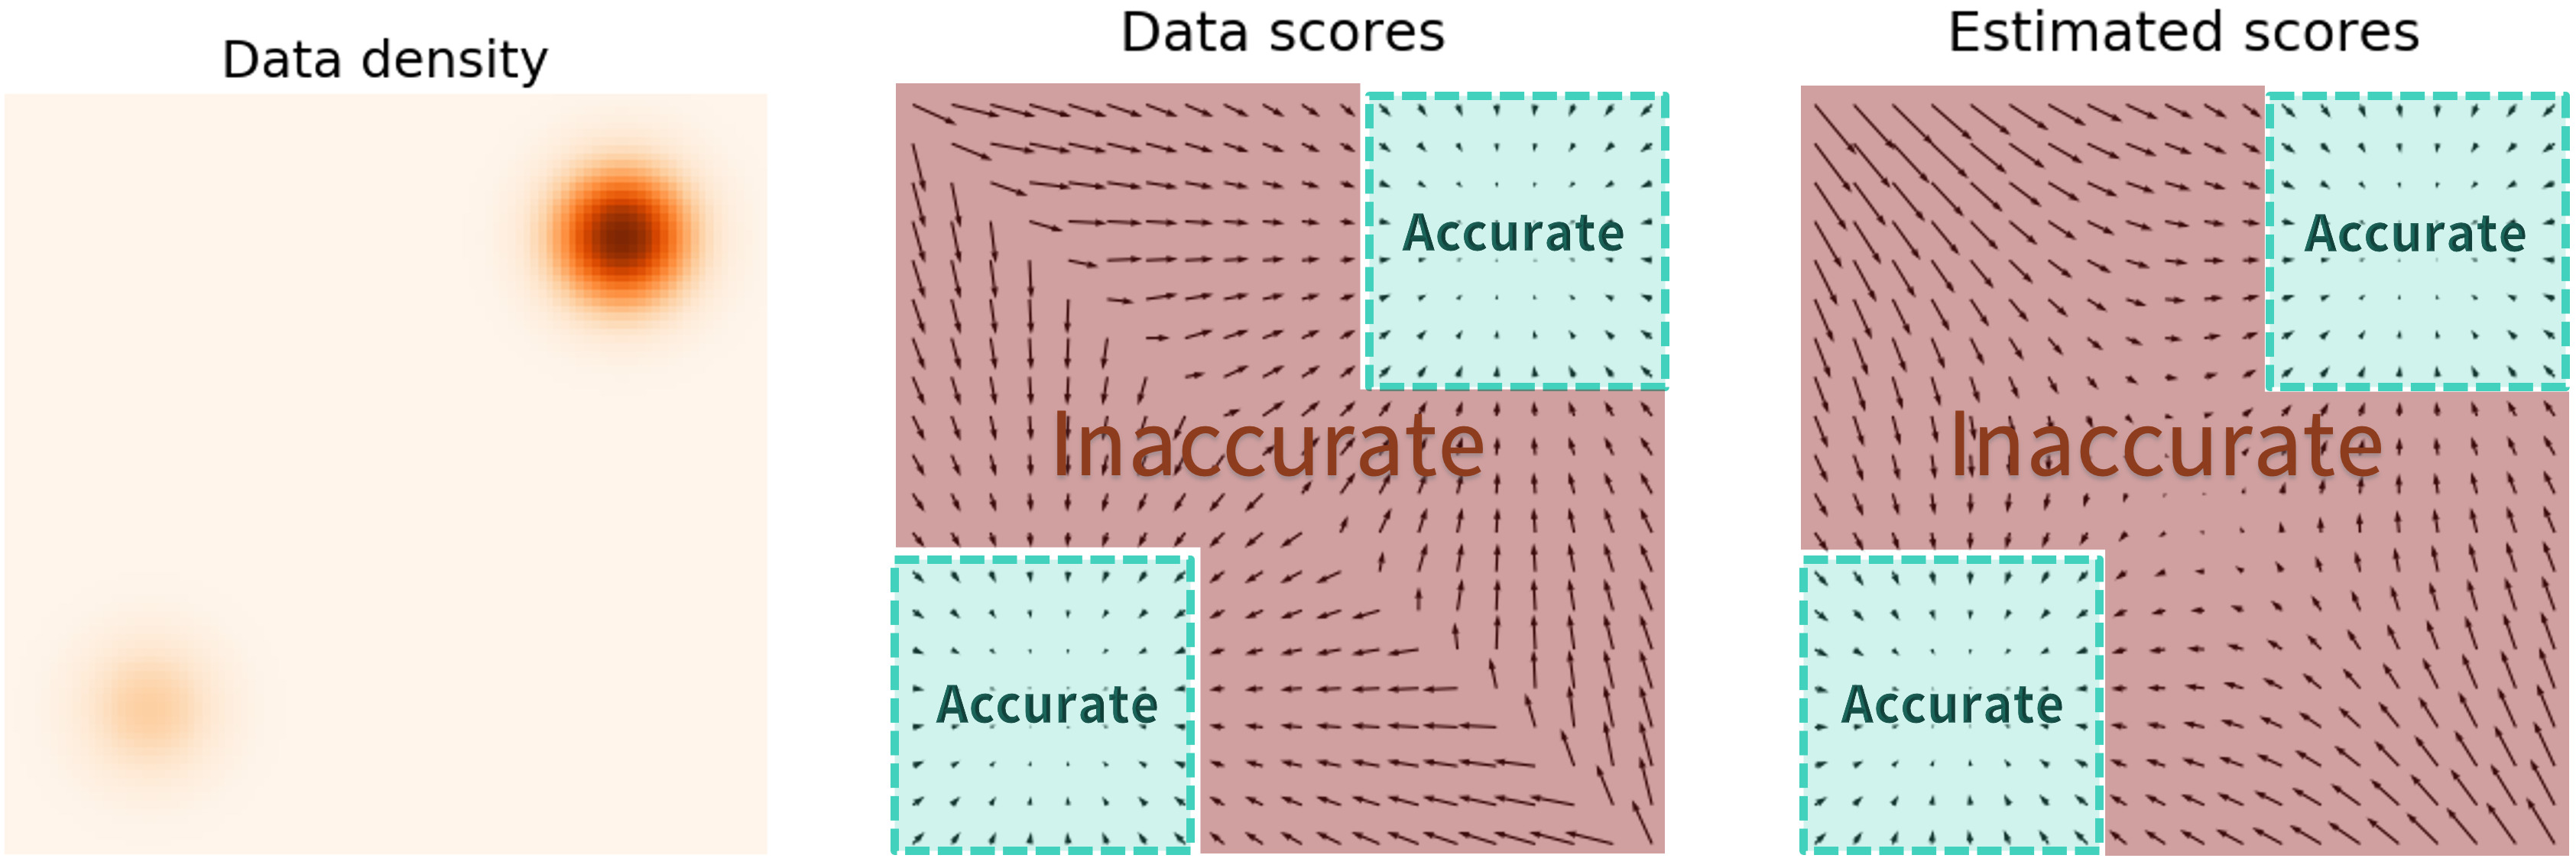
\includegraphics[width=0.75\linewidth]{figs/pitfalls}
		\end{figure}
		\item If $\sigma$ is \textbf{large}, it is good for low-density regions and  multimodal distributions, but we will learn too corrupted distribution.
		\begin{figure}
			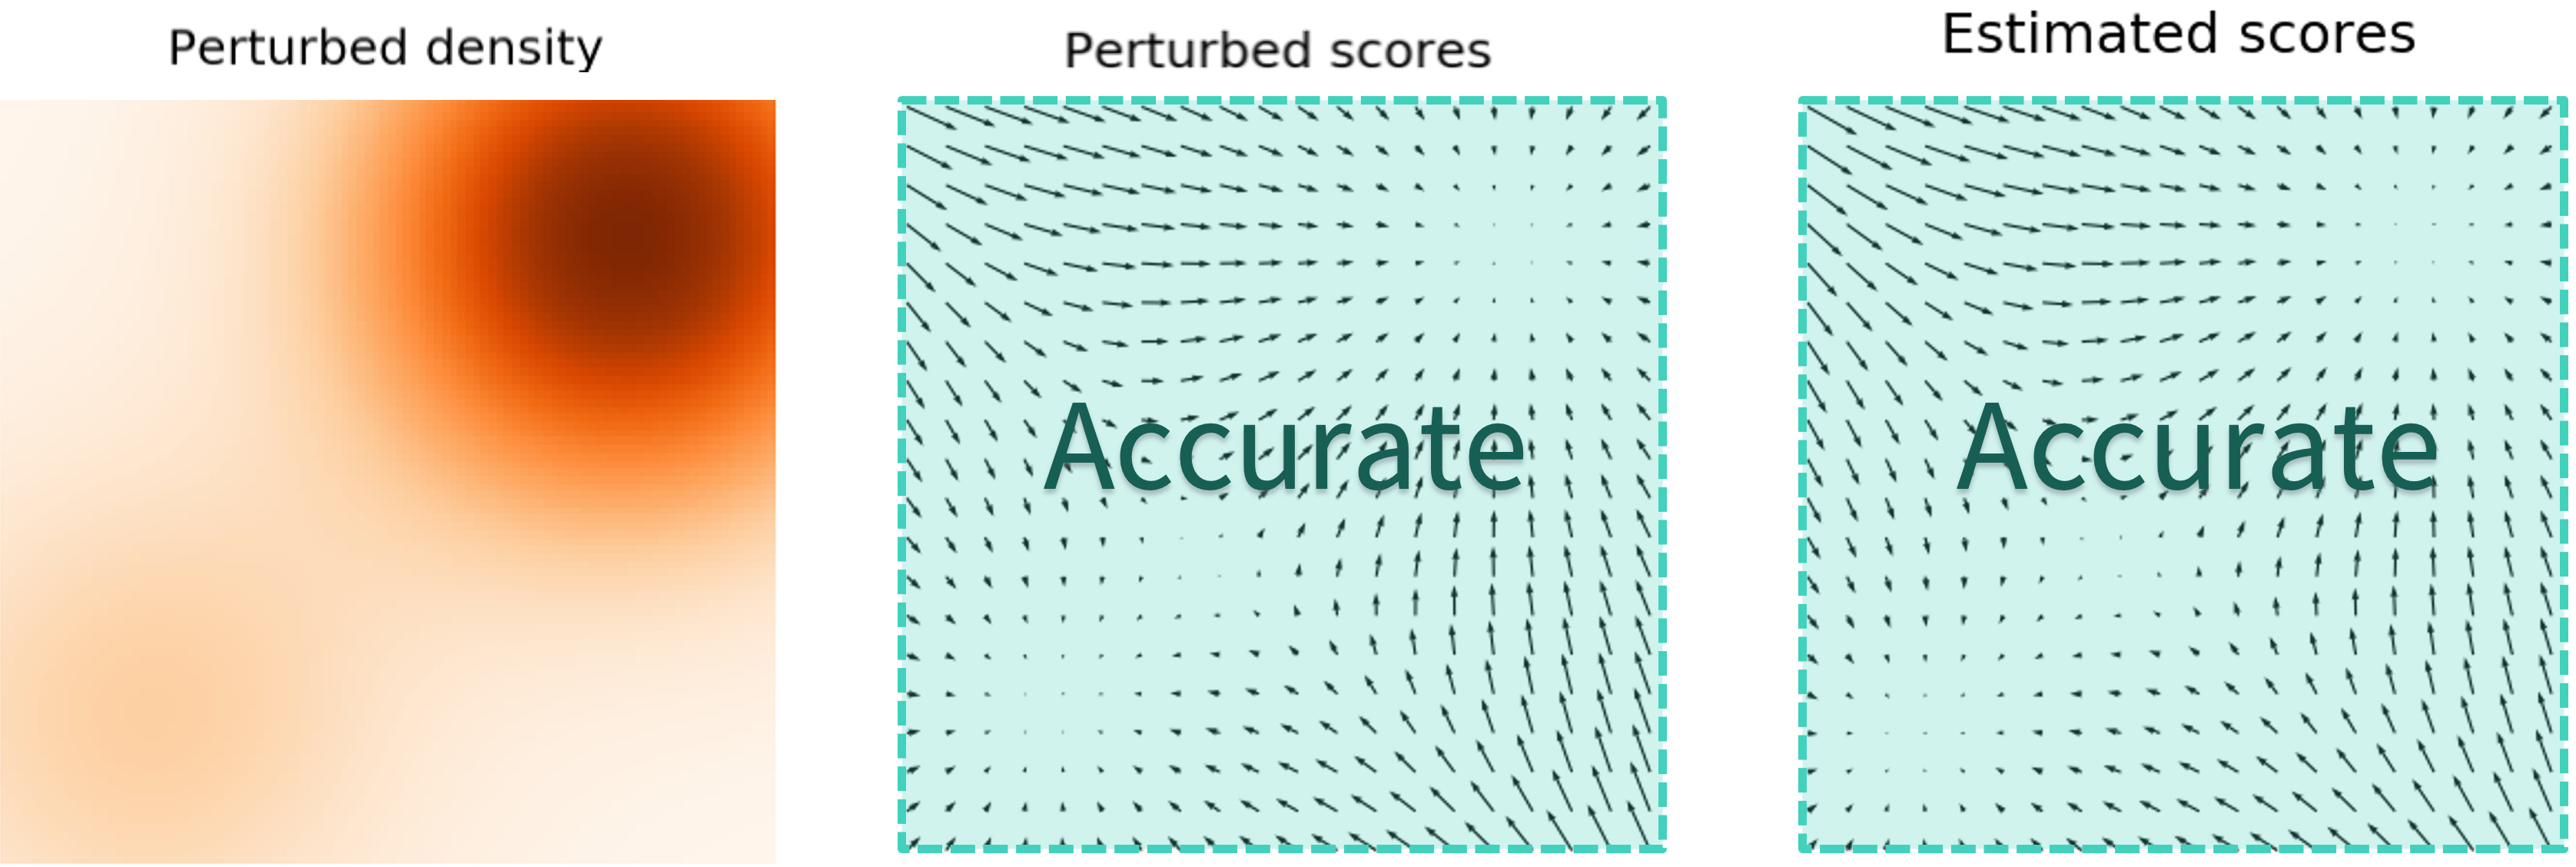
\includegraphics[width=0.75\linewidth]{figs/single_noise}
		\end{figure}
	\end{itemize}
	\myfootnotewithlink{https://yang-song.github.io/blog/2019/ssm/}{Song Y. Generative Modeling by Estimating Gradients of the Data Distribution, blog post, 2021}
\end{frame}
%=======
\begin{frame}{Noise conditioned score network}
	\begin{itemize}
		\item Define the sequence of noise levels: $\sigma_1 > \sigma_2 > \dots > \sigma_L$.
		\item Perturb the original data with the different noise level to get $\pi(\bx | \sigma_1), \dots, \pi(\bx | \sigma_L)$.
		\item Train denoised score function $\bs(\bx, \btheta, \sigma)$ for each noise level:
		\vspace{-0.2cm}
		\[
			\sum_{l=1}^L {\color{violet}\sigma_l^2} \bbE_{\pi(\bx')} \bbE_{p(\bx | \bx', \sigma_l)}\bigl\| \bs(\bx, \btheta, \sigma_l) - \nabla_\bx \log p(\bx | \bx', \sigma_l) \bigr\|^2_2 \rightarrow \min_{\btheta}
		\]
		\item Sample from \textbf{annealed} Langevin dynamics (for $l=1, \dots, L$).
	\end{itemize}
	\begin{figure}
		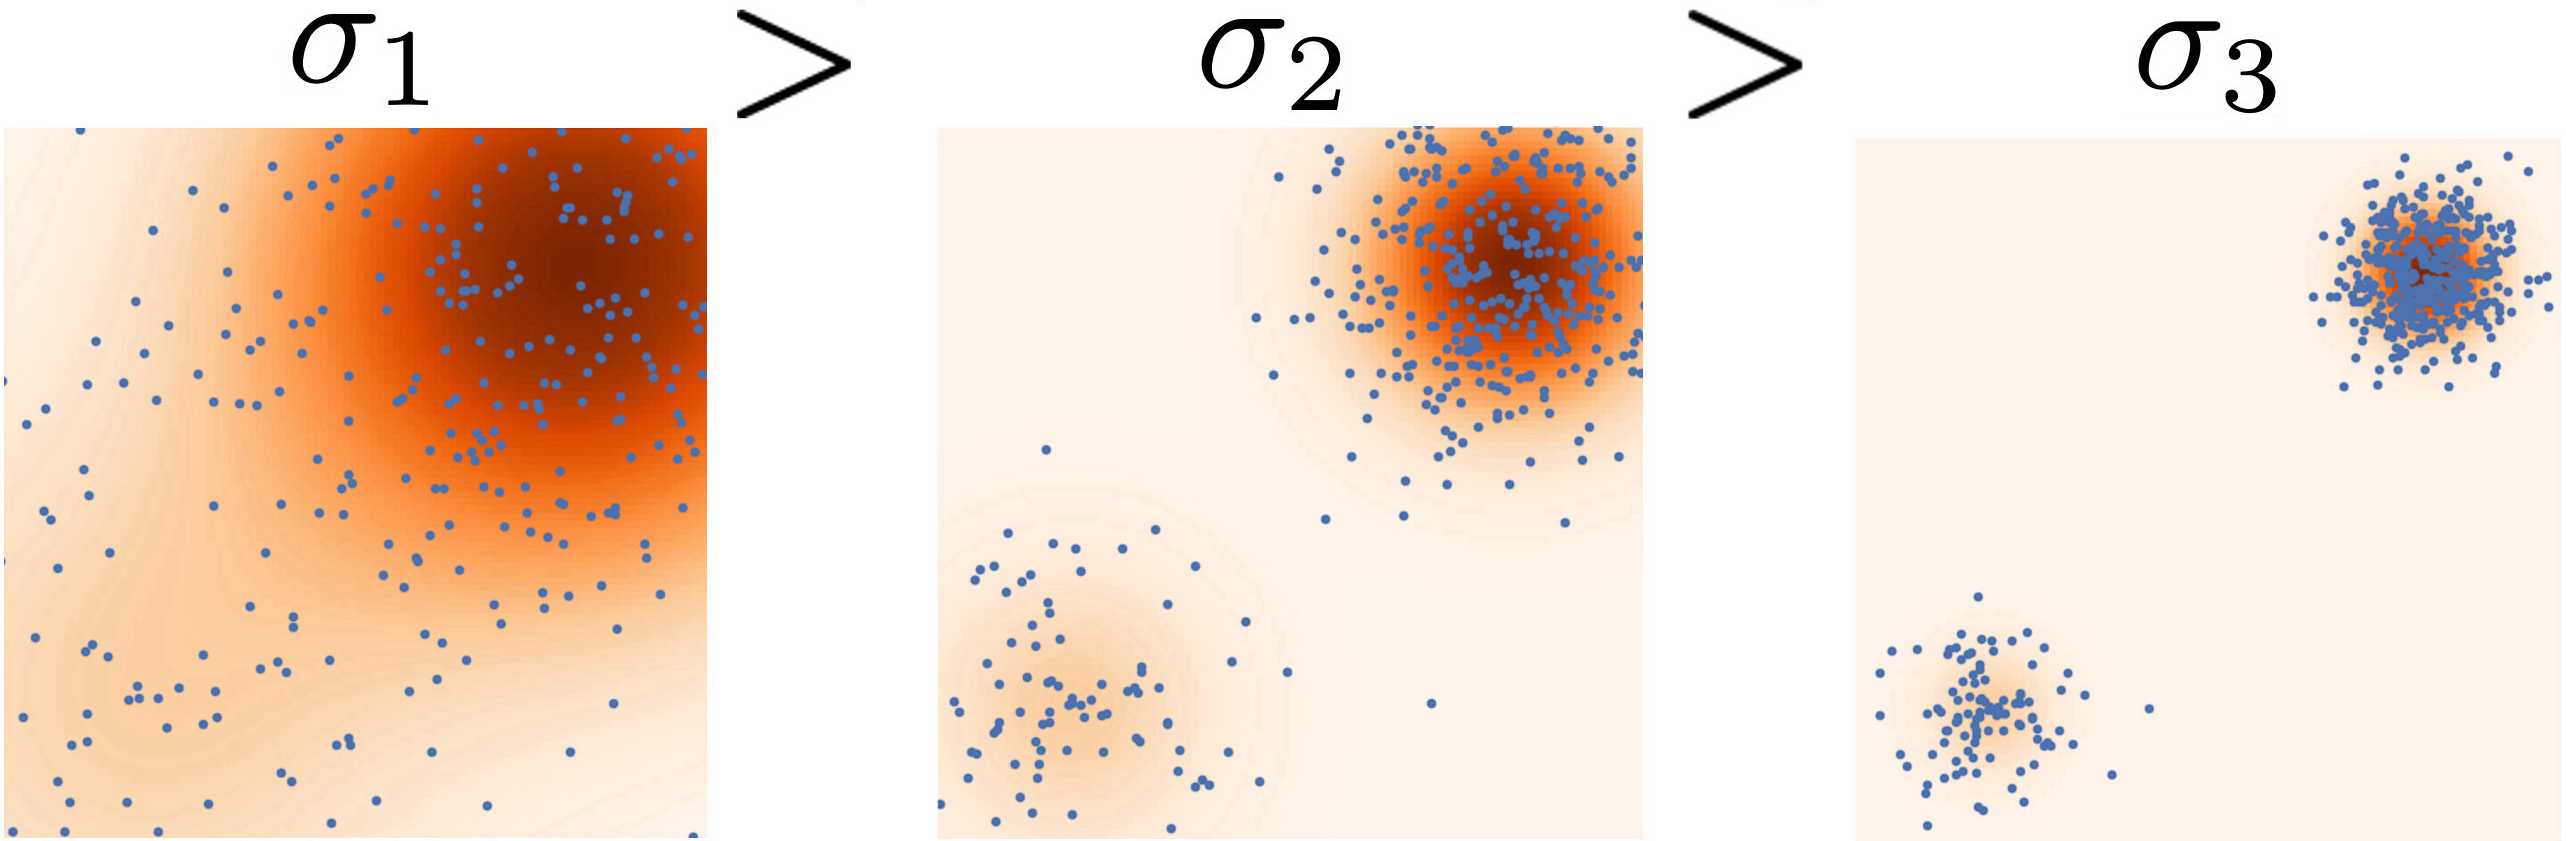
\includegraphics[width=0.6\linewidth]{figs/multi_scale}
	\end{figure}
	\begin{figure}
		
\includegraphics[width=\linewidth]{figs/duoduo}
	\end{figure}
	\myfootnotewithlink{https://arxiv.org/abs/1907.05600}{Song Y. et al. Generative Modeling by Estimating Gradients of the Data Distribution, 2019}
\end{frame}
%=======
\begin{frame}{Noise conditioned score network}
	
	\begin{minipage}{0.5\linewidth}
		\vspace{-0.7cm}
		\begin{block}{Training: loss function}
			\vspace{-0.8cm}
			\[
			\sum_{i=1}^L \sigma_l^2\bbE_{\pi(\bx')} \bbE_{\bepsilon}\left\| \bs_l + \frac{\bepsilon}{\sigma_l} \right\|^2_2,
			\]
		\end{block}
		\vspace{-0.5cm}
		Here
		\begin{itemize}
			\item $\bs_l = \bs(\bx' + \sigma_l \cdot \bepsilon, \btheta, \sigma_l)$.
			\item $\nabla_{\bx} \log p(\bx | \bx', \sigma) = - \frac{\bx - \bx'}{\sigma^2} = - \frac{\bepsilon}{\sigma_l}$.
		\end{itemize}
	\end{minipage}%
	\begin{minipage}{0.5\linewidth}
		\begin{block}{Inference: annealed Langevin dynamic}
			\begin{figure}
				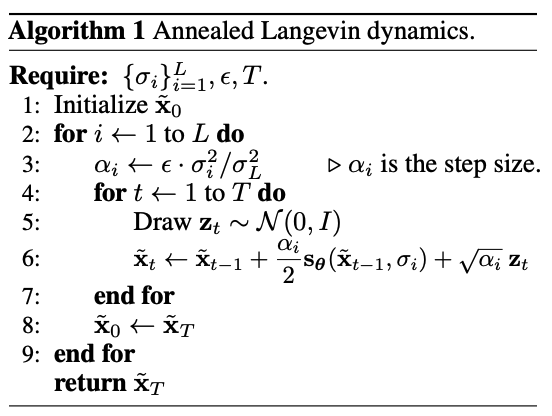
\includegraphics[width=0.9\linewidth]{figs/ald}
			\end{figure}
		\end{block}
	\end{minipage}
	\vspace{-0.7cm}
	\begin{block}{Samples}
		\begin{figure}
			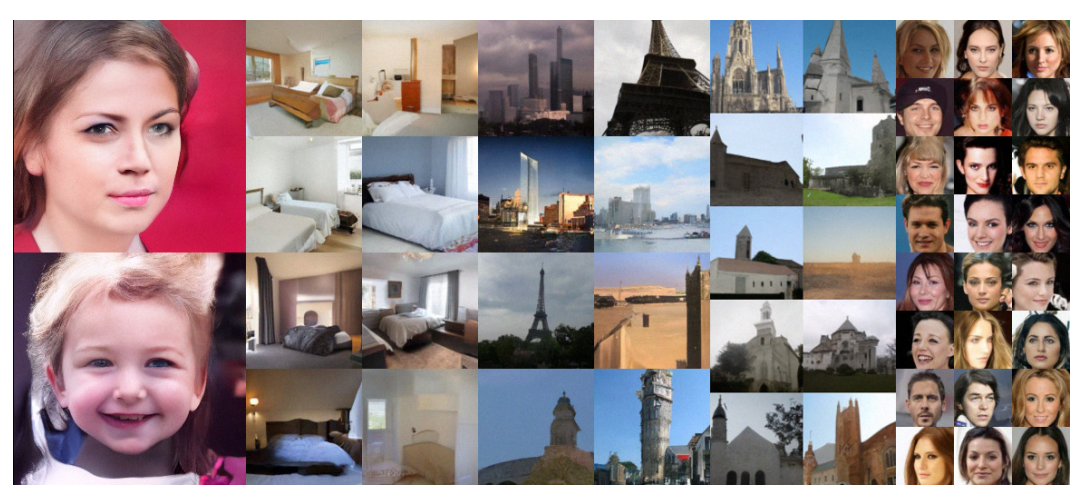
\includegraphics[width=\linewidth]{figs/NCSNv2}
		\end{figure}
	\end{block}
	\myfootnotewithlink{https://arxiv.org/abs/2006.09011}{Song Y. et al. Improved Techniques for Training Score-Based Generative Models, 2020}
\end{frame}
%=======
\section{Diffusion models}
%=======
\subsection{Gaussian diffusion process}
%=======
\begin{frame}{Forward gaussian diffusion process}
	Let $\bx_0 = \bx \sim \pi(\bx)$, $\beta \in (0, 1)$. Define the Markov chain
	\[
		\bx_t = \sqrt{1 - \beta} \cdot \bx_{t - 1} + \sqrt{\beta} \cdot \bepsilon, \quad \text{where }\bepsilon \sim \cN(0, 1);
	\]
	\[
		q(\bx_t | \bx_{t-1}) = \cN(\bx_t | \sqrt{1 - \beta} \cdot \bx_{t-1}, \beta \cdot \bI).
	\]
	\vspace{-0.6cm}
	\begin{block}{Statement 1}
		Applying the Markov chain to samples from any $\pi(\bx)$ we will get $\bx_{\infty} \sim p_{\infty}(\bx) = \cN(0, 1)$. Here $p_{\infty}(\bx)$ is a \textbf{stationary} distribution:
		\vspace{-0.2cm}
		\[
			p_{\infty}(\bx) = \int q(\bx | \bx') p_{\infty}(\bx') d \bx'. 
		\]
		\vspace{-0.8cm}
	\end{block}
	\begin{block}{Statement 2}
		Denote $\bar{\alpha}_t = \prod_{s=1}^t (1 - \beta_s)$. Then 
		\vspace{-0.2cm}
		\[
			\bx_t = \sqrt{\bar{\alpha}_t} \cdot \bx_{0} + \sqrt{1 - \bar{\alpha}_t} \cdot \bepsilon, \quad \text{where } \bepsilon \sim \cN(0, 1)
		\]
		\vspace{-0.7cm}
		\[
			q(\bx_t | \bx_0) = \cN(\bx_t | \sqrt{\bar{\alpha}_t} \cdot \bx_0, (1 - \bar{\alpha}_t) \cdot \bI).
		\]
		We could sample from any timestamp using only $\bx_0$!
	\end{block}
	\myfootnotewithlink{http://proceedings.mlr.press/v37/sohl-dickstein15.pdf}{Sohl-Dickstein J. Deep Unsupervised Learning using Nonequilibrium Thermodynamics, 2015}
\end{frame}
%=======
\begin{frame}{Forward gaussian diffusion process}
	\textbf{Diffusion} refers to the flow of particles from high-density regions towards low-density regions.
	\vspace{-0.2cm}
	\begin{figure}
		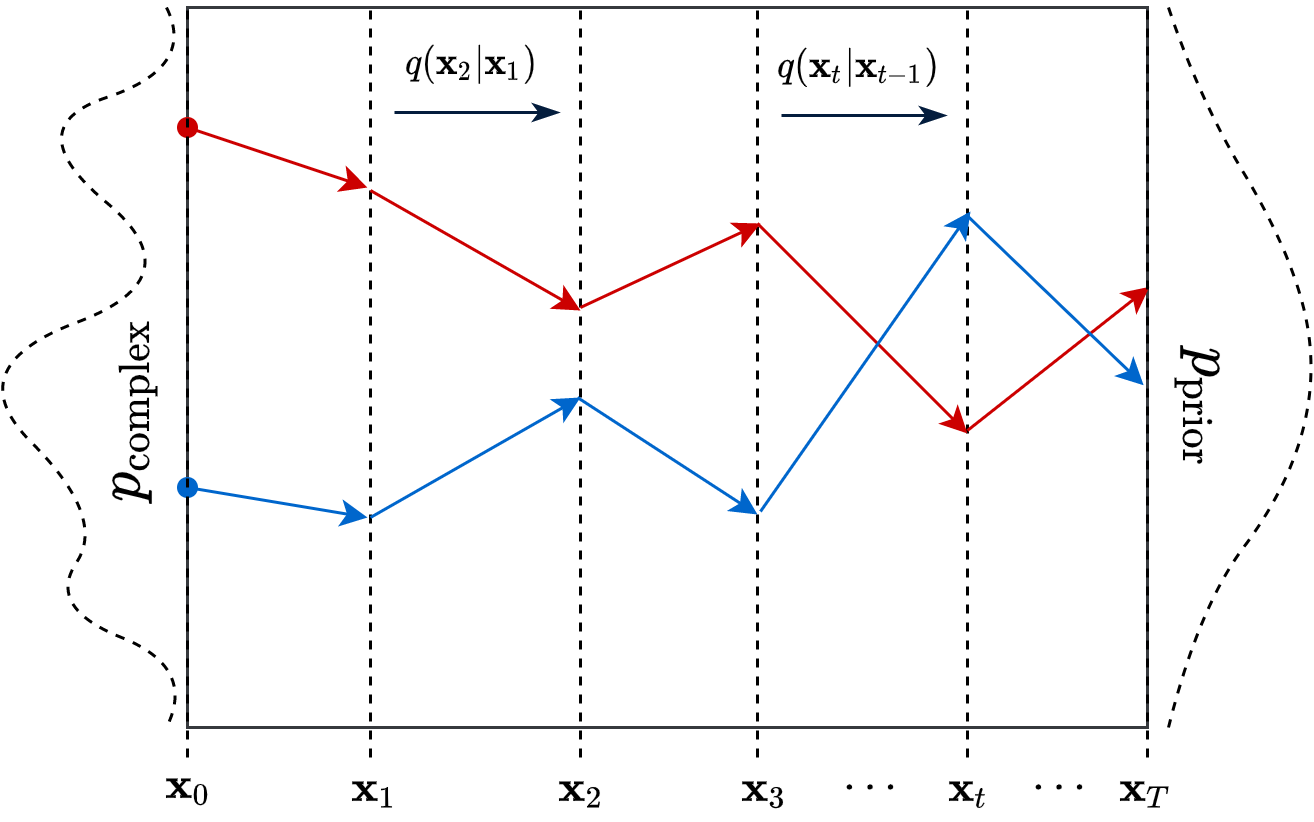
\includegraphics[width=0.5\linewidth]{figs/diffusion_over_time}
	\end{figure}
	\vspace{-0.6cm}
	\begin{enumerate}
		\item $\bx_0 = \bx \sim \pi(\bx)$;
		\item $\bx_t = \sqrt{1 - \beta} \cdot \bx_{t - 1} + \sqrt{\beta} \cdot \bepsilon$, where $\bepsilon \sim \cN(0, 1)$, $t \geq 1$;
		\item $\bx_T \sim p_{\infty}(\bx) = \cN(0, 1)$, where $T >> 1$.
	\end{enumerate}
	If we are able to invert this process, we will get the way to sample $\bx \sim \pi(\bx)$ using noise samples $p_{\infty}(\bx) = \cN(0, 1)$. \\ 
	Now our goal is to revert this process.
	\myfootnotewithlink{https://ayandas.me/blog-tut/2021/12/04/diffusion-prob-models.html}{Das A. An introduction to Diffusion Probabilistic Models, blog post, 2021}
\end{frame}
%=======
\begin{frame}{Reverse gaussian diffusion process}
	\vspace{-0.3cm} 
	\begin{figure}
		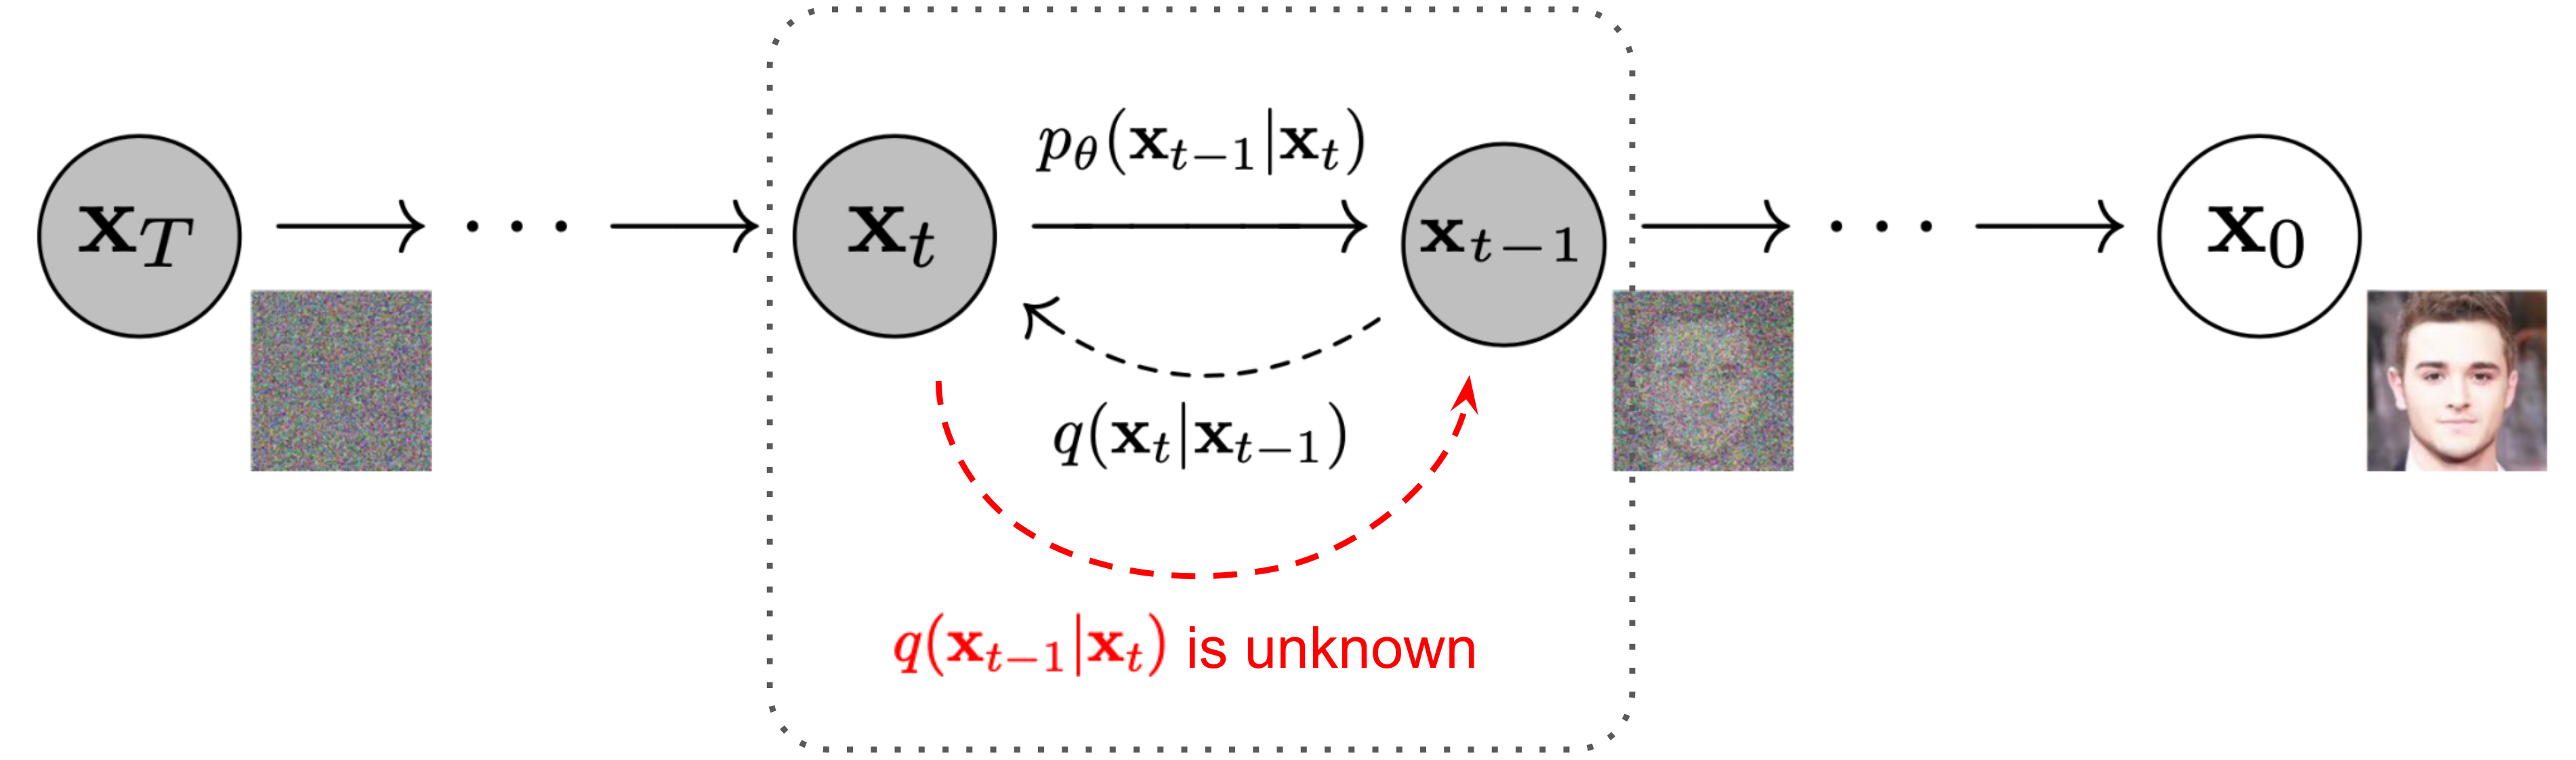
\includegraphics[width=0.8\linewidth]{figs/DDPM}
	\end{figure}
	\vspace{-0.3cm} 
	Let define the reverse process
	\vspace{-0.2cm}
	\[
		p(\bx_{t - 1} | \bx_t, \btheta) = \cN \bigl(\bx_{t - 1} | \bmu(\bx_t, \btheta, t), \bsigma^2(\bx_t, \btheta, t)\bigr)
	\]
	\vspace{-0.5cm}
	\begin{minipage}{0.5\linewidth}
		\begin{block}{Forward process}
			\begin{enumerate}
				\item $\bx_0 = \bx \sim \pi(\bx)$;
				\item $\bx_t = \sqrt{1 - \beta} \cdot \bx_{t - 1} + \sqrt{\beta} \cdot \bepsilon$, where $\bepsilon \sim \cN(0, 1)$, $t \geq 1$;
				\item $\bx_T \sim p_{\infty}(\bx) = \cN(0, 1)$.
			\end{enumerate}
		\end{block}
	\end{minipage}%
	\begin{minipage}{0.5\linewidth}
		\begin{block}{Reverse process}
			\begin{enumerate}
				\item $\bx_T \sim p_{\infty}(\bx) = \cN(0, 1)$;
				\item $\bx_{t - 1} = \bsigma(\bx_t, \btheta, t) \cdot \bepsilon + \bmu(\bx_t, \btheta, t)$;
				\item $\bx_0 = \bx \sim \pi(\bx)$;
			\end{enumerate}
		\end{block}
	\end{minipage}
	\textbf{Note:} The forward process does not have any learnable parameters!
	\myfootnotewithlink{https://lilianweng.github.io/posts/2021-07-11-diffusion-models/}{Weng L. What are Diffusion Models?, blog post, 2021}
\end{frame}
%=======
\subsection{Denoising diffusion probabilistic model (DDPM)}
%=======
\begin{frame}{Gaussian diffusion model as VAE}
	\vspace{-0.2cm}
	\begin{figure}
		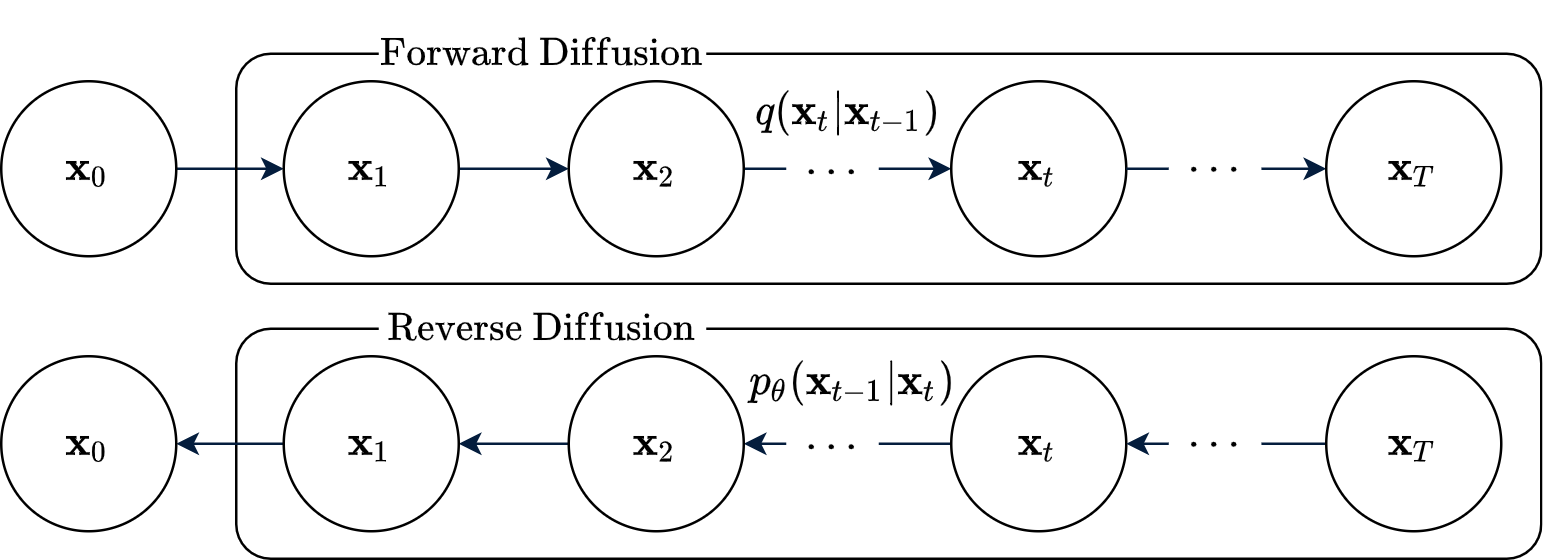
\includegraphics[width=0.65\linewidth]{figs/diffusion_pgm}
	\end{figure}
	\begin{itemize}
		\item Let treat $\bz = (\bx_1, \dots, \bx_T)$ as a latent variable (\textbf{note:} each $\bx_t$ has the same size).
		\item Variational posterior distribution (\textbf{note:} there is no learnable parameters)
		\vspace{-0.4cm}
		\[
			q(\bz | \bx) = q(\bx_1, \dots, \bx_T | \bx_0) = \prod_{t = 1}^T q(\bx_t | \bx_{t - 1}).
		\]
		\vspace{-0.5cm}
		\item Probabilistic model
		\vspace{-0.2cm}
		\[
			p(\bx, \bz | \btheta) = p(\bx | \bz, \btheta) p(\bz | \btheta)
		\]
		\item Generative distribution and prior
		\vspace{-0.3cm}
		\[
			p(\bx | \bz, \btheta) = p(\bx_0 | \bx_1, \btheta); \quad 
			p(\bz | \btheta) = \prod_{t=2}^T p(\bx_{t - 1} | \bx_t, \btheta)
		\]
	\end{itemize}
	\myfootnotewithlink{https://ayandas.me/blog-tut/2021/12/04/diffusion-prob-models.html}{Das A. An introduction to Diffusion Probabilistic Models, blog post, 2021}
\end{frame}
%=======
\begin{frame}{Gaussian diffusion model as VAE}
	\begin{block}{ELBO}
		\vspace{-0.4cm}
		\[
			\log p(\bx | \btheta) \geq \bbE_{q({\color{teal}\bz} | \bx)} \frac{p(\bx, {\color{teal}\bz} | \btheta)}{q({\color{teal}\bz} | \bx)} = \cL(q, \btheta) \rightarrow \max_{q, \btheta}
		\]
		\vspace{-0.5cm}
	\end{block}
	\begin{block}{Statement}
		\vspace{-0.8cm}
		\begin{multline*}
			\cL(q, \btheta) = \bbE_{q({\color{teal}\bx_1, \dots, \bx_T} | \bx_0)}\frac{p(\bx_0, {\color{teal}\bx_1, \dots, \bx_T} | \btheta)}{q({\color{teal}\bx_1, \dots, \bx_T} | \bx_0)} = \\ 
			= \bbE_{q} \Bigl[ {\color{violet}KL\bigl(q(\bx_T | \bx_0) || p(\bx_T)\bigr)}
			+ \sum_{t=2}^T \underbrace{KL \bigl(q(\bx_{t-1} | \bx_t, \bx_0) || p(\bx_{t - 1} | \bx_t, \btheta )\bigr)}_{\cL_t} - \\
			- {\color{olive}\log p(\bx_0 | \bx_1, \btheta)} \Bigr]
		\end{multline*}
		\vspace{-0.5cm}
	\end{block}
	\begin{itemize}
		\item {\color{violet}First term} is constant (KL between two standard normals).
		\item {\color{olive}Third term} is a decoder distribution (could be AR model or discretized distribution (like mixture of logistics)). 
	\end{itemize}
	\myfootnotewithlink{https://arxiv.org/abs/2006.11239}{Ho J. Denoising Diffusion Probabilistic Models, 2020}
\end{frame}
%=======
\begin{frame}{Gaussian diffusion model as VAE}
	\[
		\cL_t = {\color{teal}KL \bigl(q(\bx_{t-1} | \bx_t, \bx_0) || p(\bx_{t - 1} | \bx_t, \btheta )\bigr)}.
	\]
	Here
	\[
		q(\bx_{t-1} | \bx_t, \bx_0) = \cN(\bx_{t-1} | \tilde{\bmu}_t(\bx_t, \bx_0), \tilde{\beta}_t \bI),
	\]
	$\tilde{\bmu}_t(\bx_t, \bx_0)$ and $\tilde{\beta}_t$ have analytical formulas (we omit it) and both dependent on $\beta_t$.
	\begin{itemize}
		\item \textbf{Note:} We do not have an analytical expression for $q(\bx_{t-1} | \bx_t)$.
		\item Assume $\bsigma^2(\bx_t, \btheta, t) = \tilde{\beta}_t \bI$ {\color{gray}(reminder: $p(\bx_{t - 1} | \bx_t, \btheta) = \cN(\bx_{t - 1} | \bmu(\bx_t, \btheta, t), \bsigma^2(\bx_t, \btheta, t))$)}.
		\item Use KL formula between two normal distributions:
		\begin{align*}
			\cL_t &= KL\Bigl(\cN\bigl(\tilde{\bmu}_t(\bx_t, \bx_0), \tilde{\beta}_t \bI \bigr) || \cN\bigl(\bmu(\bx_t, \btheta, t), \tilde{\beta}_t \bI\bigr)\Bigr) \\ 
			&= \bbE_{\bepsilon} \left[ \frac{1}{2\tilde{\beta}_t} \bigl\| \tilde{\bmu}_t(\bx_t, \bx_0) - \bmu(\bx_t, \btheta, t) \bigr\|^2 \right]
		\end{align*}
	\end{itemize}
	\myfootnotewithlink{https://arxiv.org/abs/2006.11239}{Ho J. Denoising Diffusion Probabilistic Models, 2020}
	\end{frame}
%=======
\begin{frame}{Gaussian diffusion model as VAE}
	\begin{multline*}
		\cL_t = \bbE_{\bepsilon} \left[ \frac{1}{2\tilde{\beta}_t} \| {\color{violet} \tilde{\bmu}_t(\bx_t, \bx_0)} - \bmu(\bx_t, \btheta, t) \|^2 \right] = \\ 
		= \bbE_{\bepsilon} \left[ \frac{1}{2\tilde{\beta}_t} \left\| {\color{violet} \frac{1}{\sqrt{1 - \beta_t}}\left( \bx_t - \frac{\beta_t}{\sqrt{1 - \bar{\alpha}_t} } \bepsilon \right)} - \bmu(\bx_t, \btheta, t) \right\|^2 \right]
	\end{multline*}
    {\color{gray}Here we used the analytic expression for $\tilde{\bmu}_t(\bx_t, \bx_0)$.}
	\begin{block}{Reparametrization}
		\vspace{-0.3cm}
		\[
			\bmu(\bx_t, \btheta, t) = \frac{1}{\sqrt{1 - \beta_t}}\left( \bx_t - \frac{\beta_t}{\sqrt{1 - \bar{\alpha}_t} } \bepsilon(\bx_t, \btheta, t) \right) 
		\]
		\vspace{-0.6cm}
	\end{block}
	\begin{block}{KL term}
		\vspace{-0.2cm}
		\[
			\cL_t = \bbE_{\bepsilon} \left[ \frac{\beta_t^2}{2\tilde{\beta}_t (1 - \beta_t)} \left\| \frac{\bepsilon}{\sqrt{1 - \bar{\alpha}_t}} - \frac{\bepsilon({\color{teal}\bx_t}, \btheta, t)}{\sqrt{1 - \bar{\alpha}_t}}\right\|^2 \right]
		\]
		\[
			{\color{teal}\bx_t} = \sqrt{\bar{\alpha}_t} \cdot \bx_{0} + \sqrt{1 - \bar{\alpha}_t} \cdot \bepsilon, \quad \text{where } \bepsilon \sim \cN(0, 1)
		\]
		\vspace{-0.5cm}
	\end{block}
	\myfootnotewithlink{https://arxiv.org/abs/2006.11239}{Ho J. Denoising Diffusion Probabilistic Models, 2020}
\end{frame}
%=======
\begin{frame}{Gaussian diffusion model vs Score matching}
	\vspace{-0.3cm}
	\[
		\cL_t = {\color{olive}\bbE_{\bepsilon}} \left[ \frac{\beta_t^2}{2\tilde{\beta}_t (1 - \beta_t)} \left\| {\color{violet}\frac{\bepsilon}{\sqrt{1 - \bar{\alpha}_t}}} - {\color{teal}\frac{\bepsilon(\bx_t, \btheta, t)}{\sqrt{1 - \bar{\alpha}_t}}}\right\|^2 \right]
	\]
	\begin{itemize}
		\item Result from Statement 2
		\[
			q(\bx_t | \bx_0) = \cN(\bx_t | \sqrt{\bar{\alpha}_t} \cdot \bx_0, (1 - \bar{\alpha}_t) \cdot \bI).
		\]
		\item Score of noised distribution
		\[
			\nabla_{\bx_t} \log q(\bx_t | \bx_0) = - \frac{\bepsilon}{\sqrt{1 - \bar{\alpha}_t}}, \quad \text{where } \bepsilon \sim \cN(0, 1).
		\]
		\item Let reparametrize our model: 
		\[
			\bs(\bx_t, \btheta, t) = \frac{\bepsilon(\bx_t, \btheta, t)}{\sqrt{1 - \bar{\alpha}_t}}.
		\]
	\end{itemize}
	\begin{block}{Noise conditioned score network}
		\vspace{-0.2cm}
		\[
			{\color{olive}\bbE_{p(\bx | \bx', \sigma_l)}}\bigl\| {\color{teal}\bs(\bx, \btheta, \sigma_l)} - {\color{violet}\nabla_\bx \log p(\bx | \bx', \sigma_l)} \bigr\|^2_2 \rightarrow \min_{\btheta}
		\]
	\end{block}
	\myfootnotewithlink{https://arxiv.org/abs/2006.11239}{Ho J. Denoising Diffusion Probabilistic Models, 2020}
	\end{frame}
%=======
\begin{frame}{Denoising diffusion probabilistic model (DDPM)}
	\begin{block}{Samples}
		\begin{figure}
			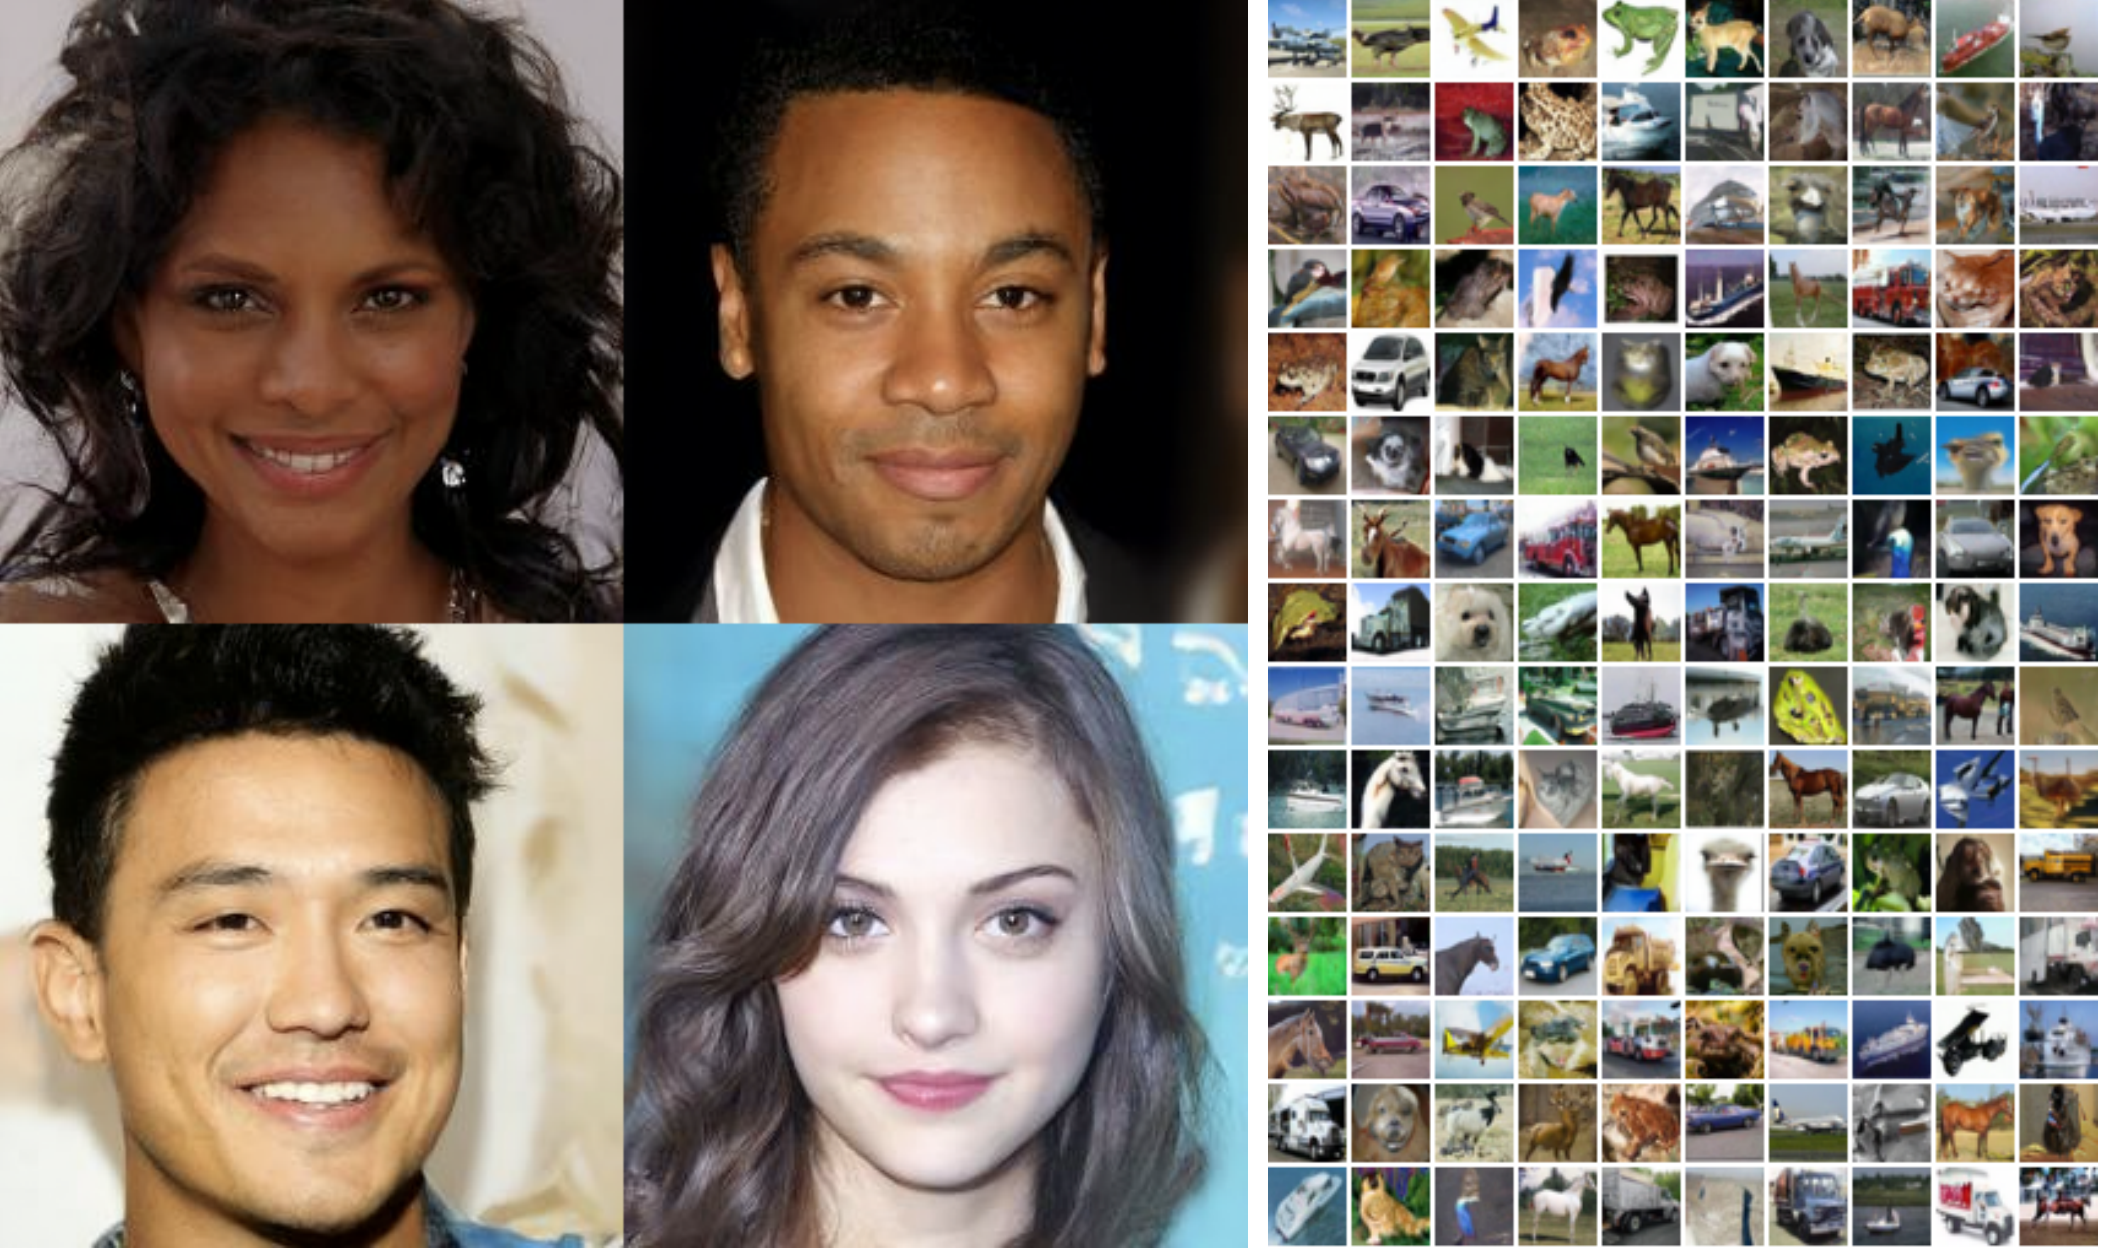
\includegraphics[width=\linewidth]{figs/ddpm_samples}
		\end{figure}
	\end{block}
	\myfootnotewithlink{https://arxiv.org/abs/2006.11239}{Ho J. Denoising Diffusion Probabilistic Models, 2020}
\end{frame}
%=======
\begin{frame}{The poorest course overview :)}
	\begin{figure}
		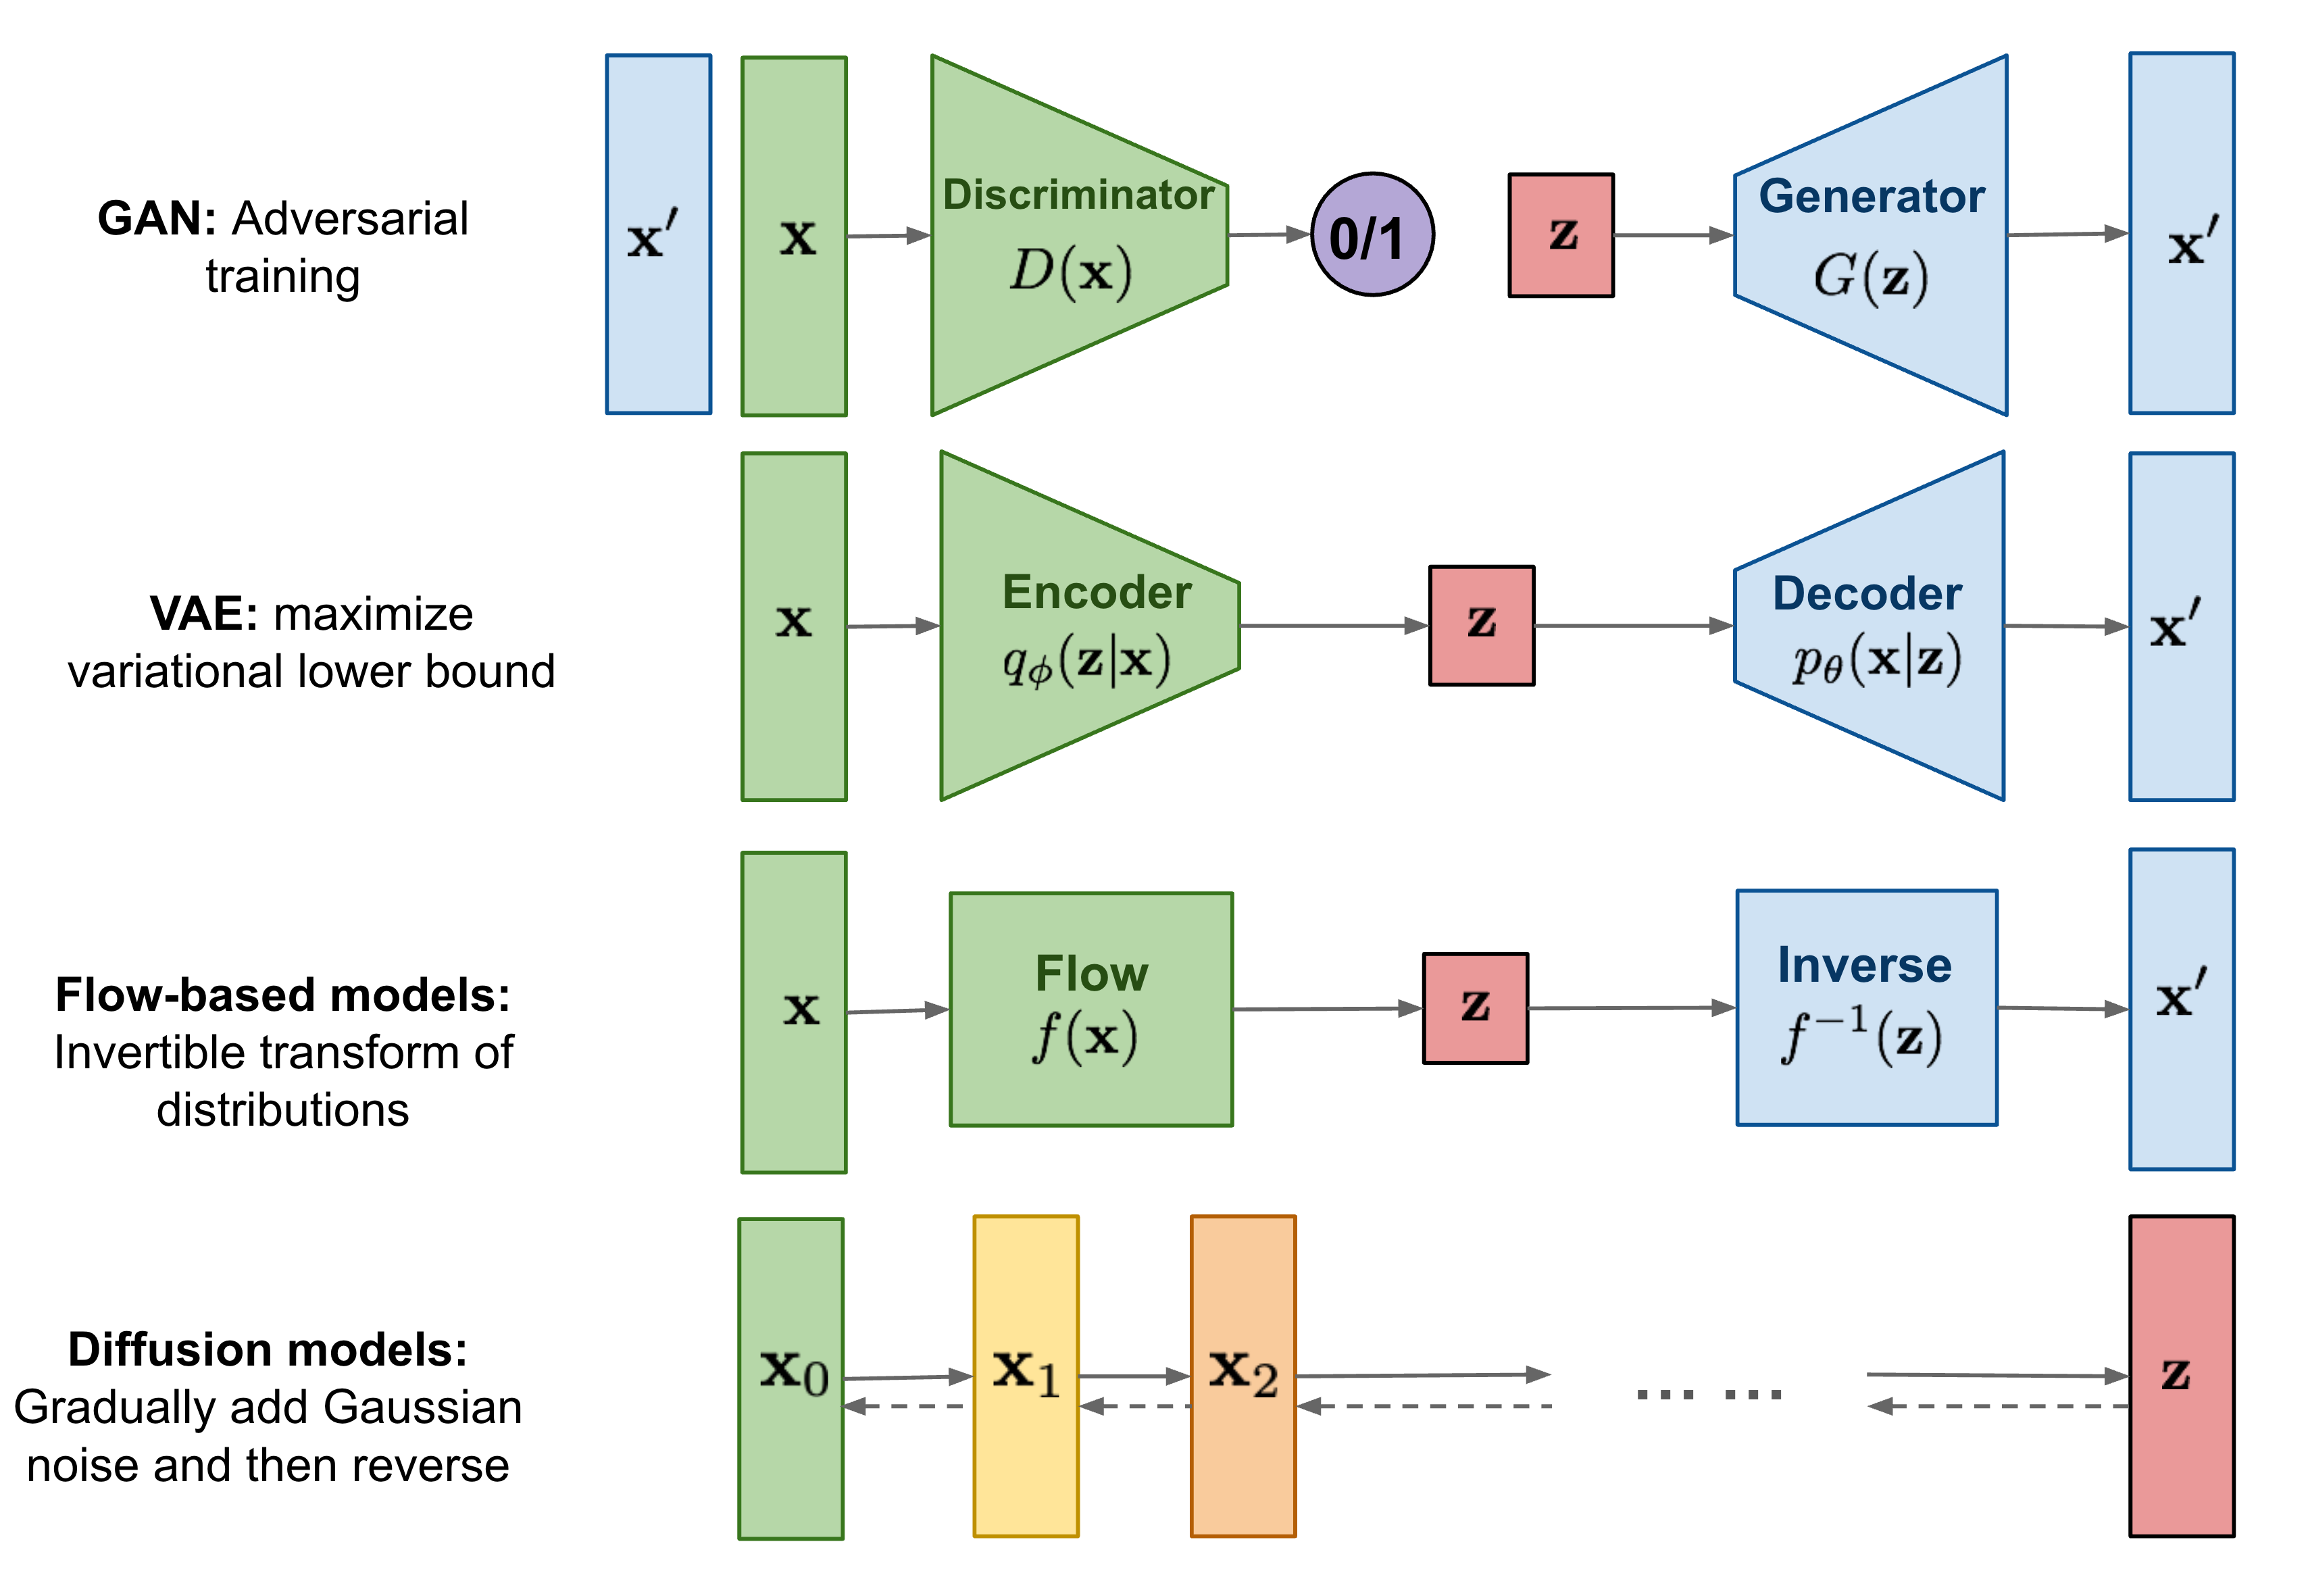
\includegraphics[width=\linewidth]{figs/generative-overview}
	\end{figure}
	\myfootnotewithlink{https://lilianweng.github.io/posts/2021-07-11-diffusion-models/}{Weng L. What are Diffusion Models?, blog post, 2021}
\end{frame}
%=======
\begin{frame}{Summary}
	\begin{itemize}
		\item Noise conditioned score network uses multiple noise levels and annealed Langevin dynamics to fit score function.
		\vfill
		\item Gaussian diffusion process is a Markov chain that injects special form of Gaussian noise to the samples.
		\vfill
		\item Reverse process allows to sample from the real distribution $\pi(\bx)$ using samples from noise.
		\vfill
		\item Diffusion model is a VAE model which reverts gaussian diffusion process using variational inference.
		\vfill
		\item Objective of diffusion model is closely related to the noise conditioned score network and score matching.
	\end{itemize}
\end{frame}
\end{document} 